\documentclass{cshonours}
\bibliographystyle{acm}

\usepackage{graphics}  %optional

\title{RNA Folding: Local Versus Global Optimization}
\author{Max Ward (20748588)}

\keywords{Honours, report, dissertation, UWA, RNA, bioinformatics}
\categories{Not, really, sure}

\begin{document}
\maketitle

\begin{abstract}
I am definitely going to need to write this at some point. This is a short report on how to use the {\tt cshonours.cls} class
to prepare dissertations using the latest \LaTeX\ version,
\LaTeX2e. This class is based on the standard class {\tt report.cls}.
\end{abstract}

\begin{acknowledgements}
Going to need something here too.
This class is designed to produce reports that look
the same as those produced by the older {\tt cshonours.sty} style for
\LaTeX 2.09, which was modified by Nick Spadaccini from a style
provided by Ken Wessen.
\end{acknowledgements}

\tableofcontents
\listoftables  %optional
\listoffigures  %optional



\chapter{Introduction}
\section{DNA and RNA}
Deoxyribonucleic Acid (DNA) is the basic genetic building block upon which the classification of genetic material into genes and chromosomes is based. The role of DNA as the hereditary unit of genetics was determined in the 1940s \cite{albertsessential}. Soon thereafter, Watson \& Crick \cite{watson1953molecular} published a highly acclaimed paper describing the fundamental chemical structure of DNA. In it, they outlined a double helix formation which has since become as iconic as it is canonical (see Figure \ref{dna}). Each strand of the helix Watson \& Crick discovered is essentially a chain of `nucleotides' which are made of a sugar-phosphate backbone, attached to a single `base'. The bases of each strand form hydrogen bonds which hold the double helix together. The most astonishing and important of their findings was that these bases bond in a reciprocal fashion. They described four bases: Adenine (A), which always bonds to Thymine (T), and Guanine (G), which always bonds to Cytosine (C).

\begin{figure}
\begin{center}
\scalebox{0.23}{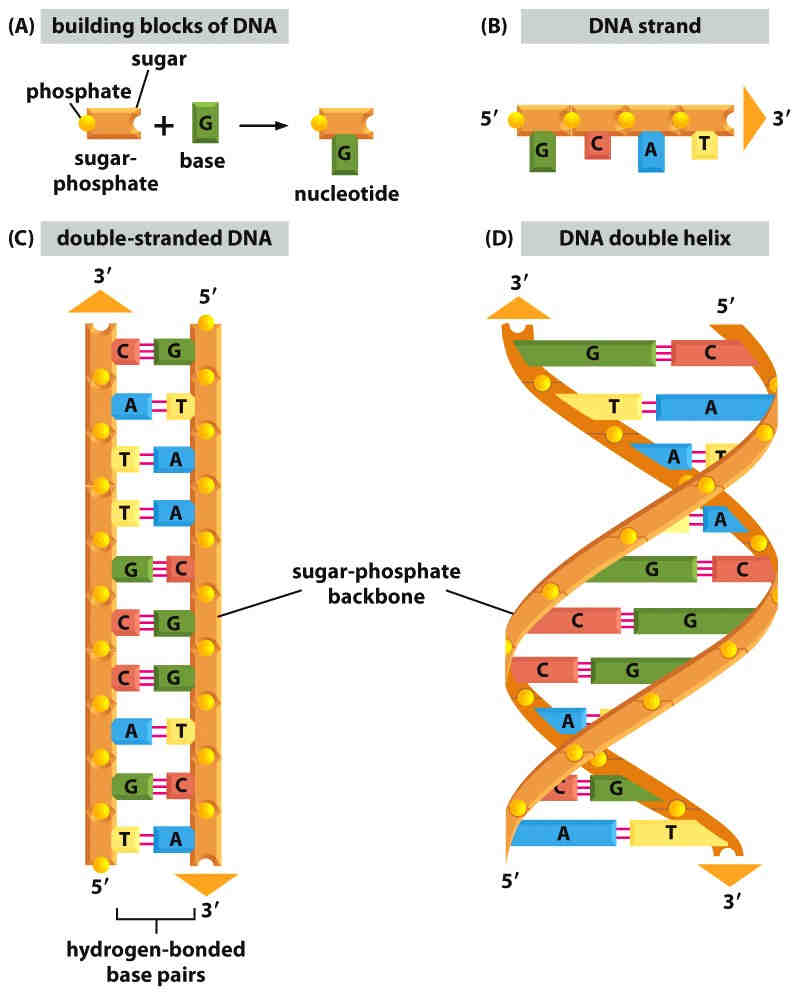
\includegraphics{dna}}
\end{center}
\caption{The structure and composition of DNA. Diagram taken from "Essential Cell Biology" \cite{albertsessential}.}
\label{dna}
\end{figure}

The reciprocal bonding relationships between bases is what allows replication to occur; a copy of the DNA can be made by simply allowing the correct bases to bond to one of the strands making up its helix. This gives a model for inheritance and cellular replication. However, there remains the question of how DNA can actually code for protein. Proteins are made up amino acids bonded in a specific sequence \cite{albertsessential}. The DNA must therefore code for amino acids. This code, which can be thought of as the `digital' representation for the `analogue' protein used by our cells, needs to be carried to ribosomes which translate it into protein \cite{albertsessential}. This is a task carried out by Ribonucleic Acid (RNA). RNA is very much like DNA in that it can bond reciprocally to another strand with matching bases. The main difference is that it is single stranded in structure, and has Uracil (U) in place of Thymine \cite{albertsessential}. It is important to note that in RNA molecules G and U pairings are also possible. RNA bonds to DNA and, in a sense, reads it. This results in the production of a copy of the DNAs genetic payload. This `downloaded' information is then carried away to be translated into protein \cite{albertsessential}. An example of this is depicted in Figure \ref{transcription}, in which we see a Messenger RNA molecule bonding to and thus making a copy of a section of DNA. As depicted in Figure \ref{transcription}, the 3' end of a DNA or RNA molecule is the end onto which new nucleotides are added. The 5' end is chemically stable, and nucleotides are not usually appended to it \cite{albertsessential}.

\begin{figure}
\begin{center}
\scalebox{0.23}{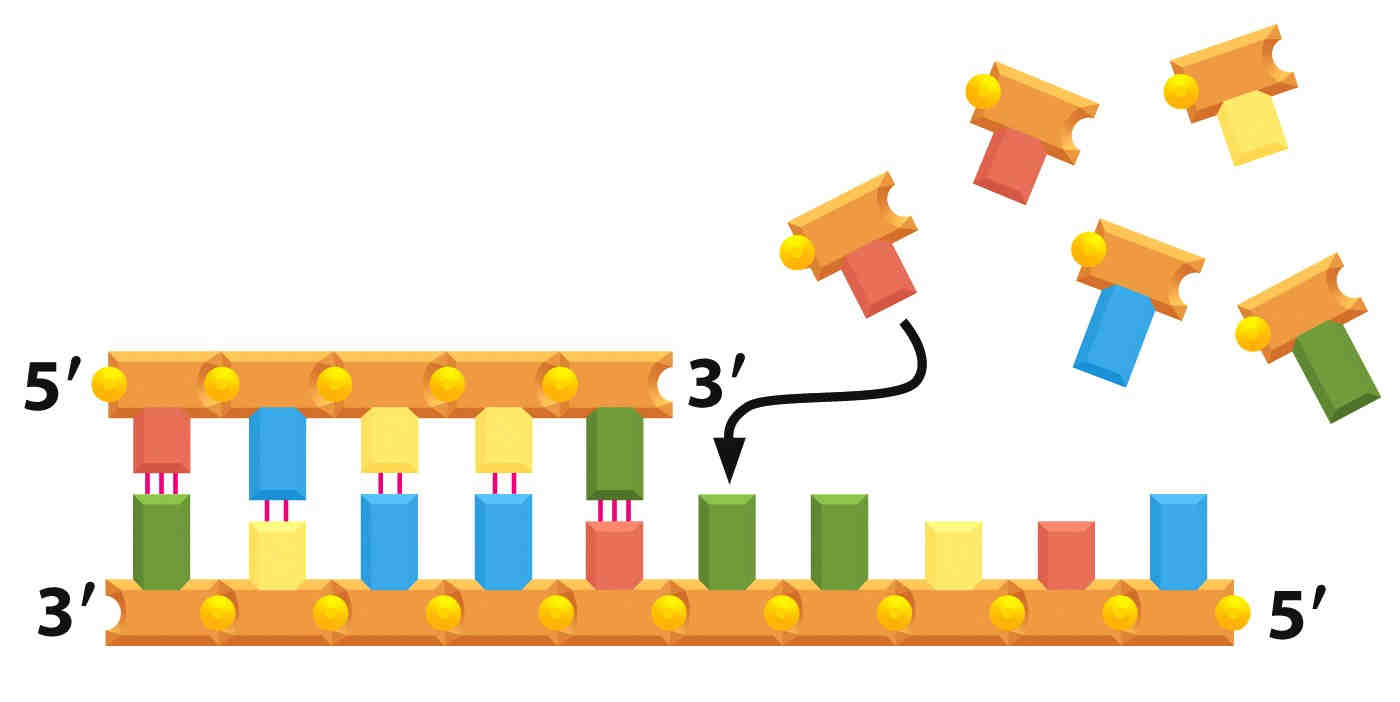
\includegraphics{transcription}}
\end{center}
\caption{RNA transcription. Diagram taken from "Essential Cell Biology" \cite{albertsessential}.}
\label{transcription}
\end{figure}



For many years the conventional wisdom was that DNA contained genes which coded for functional proteins used by the cell \cite{albertsessential}. Though this is undoubtedly true, there was a problem: much of the human genome, and the genomes of other species, contains DNA which does not appear to code for anything \cite{beaton1999eukaryotic}. Many theories have been put forward to explain this. It was argued that this `junk' DNA is the perennial build-up of mutation, and that natural selection simply cannot act with strong enough selective force to cull this free-loading DNA \cite{beaton1999eukaryotic}. Surprisingly, much of this non-coding DNA is actually transcribed into RNA, despite having no apparent function \cite{leung2013coral}. As it turns out, RNA is more than a simple messenger for encoded proteins. Recent research has found myriad important functions for RNA. For example, RNA can act as a catalyst for RNA splicing and peptide bond formation, and can also alter the regulation of genes \cite{xu2012statistical}. It seems that much of our genome contains templates for non-coding RNAs (ncRNAs). These RNAs perform essential cellular functions without actually being translated into protein at any point in their life-cycle \cite{leung2013coral}. Because of its inherently single stranded nature, RNA forms bonds with itself, folding into secondary and tertiary structures \cite{conn1998rna}.


It is axiomatic that chemical structure is tantamount to biological function; RNA is no exception. For this reason there has and continues to be an intense interest in predicting the secondary structure and tertiary structure of RNA molecules. This is in part because it will elucidate the underlying principles of RNA structure formation and function \cite{conn1998rna}, but also because it will allow the detection and classification of unknown RNAs, enable prediction of novel RNA function, and assist the design of new RNA based drugs \cite{condon2003problems}. In fact, RNA is an extremely versatile molecule, and as such is attractive from both an engineering and computational point of view. Small combinatorial computation problems have been solved by representing the solution set using RNAs. Furthermore, a theory of computation has been put forward using self assembling RNA molecules \cite{condon2003problems}. As if to comment on the upheaval of a protein-centric view of biology in recent years, researchers have found that RNA is capable of supporting all the processes required for life without the need of protein \cite{condon2003problems}. The secondary structure of RNA is also highly conserved during evolution, indicating its importance \cite{hofacker2008rna}. Secondary and tertiary structures can be treated hierarchically, as a result it is possible to predict the secondary structure of an RNA without understanding the tertiary structure. The tertiary structure in turn builds upon the secondary structure \cite{tinoco1999rna}. This paper will focus on secondary structure prediction.

It holds to reason that an algorithm for RNA secondary structure prediction can never be realised if we do not understand how these structures form, or their general morphology. For this reason it is important to understand how true RNA secondary structures can be determined, and the limitations of these techniques. DNA and RNA molecules can be analysed using X-ray crystallographic methods. These types of approaches work because the wavelengths of some X-rays are the same as the dimensions of DNA and RNA inter-atomic bonds. The diffraction of X-ray light by these molecules can thus be observed and their structures can subsequently be inferred by analysis of the resulting data. Nuclear Magnetic Resonance (NMR) is another technique which can be applied to the analysis of DNA/RNA. It relies on the spin of atoms when in a magnetic field. These spin signals can be used to determine the atomic composition and topology of a molecule. This has the advantage of not requiring the molecule under analysis to be crystallized before analysis. Arguably this gives a better in vivo view of RNAs/DNAs, which are fundamentally flexible structures. NMR also has some disadvantages; for instance, it is less accurate than X-ray crystallography, and cannot be used on extremely large molecules. The reason these techniques cannot be used for all RNA structural assays is that they are extremely expensive and time consuming \cite{neidle2010principles}.


RNA secondary structure prediction techniques can be broadly broken into two categories: those that use auxiliary information to assist in prediction, and those that predict structure ex nihilo---that is, with nothing but the `proband' sequence we require a structure for. The former approach typically does consensus matching between some sequences for which a user already knows the secondary structures, and a sequence for which the structure is unknown \cite{hofacker2008rna}. In this paper I investigate the latter approach because it requires deeper knowledge about why and how RNAs fold. Also, it is the more general of the two.



\section{Dynamic Programming Techniques}
\subsection{Fundamental Algorithms}
The first such algorithms were based on relatively naive brute force. All possible secondary structures were enumerated and the one with
the most bonds was selected as the solution \cite{nussinov1978algorithms}. While being very simplistic,
these first approaches introduce an important assumption: RNA molecules will
form energetically stable secondary structures. Maximising bonds is a crude but
nonetheless accurate measure of energetic stability, as every bond increases the
stability of a structure \cite{nussinov1978algorithms}. In the late 1970s, when the first large RNA molecules
were being successfully sequenced, Nussinov et al. \cite{nussinov1978algorithms} introduced an algorithm
based on loop matching for bonding pairs. Their algorithm attempted to find a
single structure with the maximal number of bonds using dynamic programming,
with the restriction that all bonding pairs had to be entirely nested. It did this in $O(N^3)$ time and using $O(N^2)$ space. Thence Nussinov \& Jacobson \cite{nussinov1980fast} introduced
a refined version of the same algorithm and began testing it against experimentally verified RNA secondary structures. They had mixed success; Transfer RNAs
(tRNAs) were conspicuous in their difference from predicted structures.

\begin{figure}
\begin{center}
\scalebox{0.3}{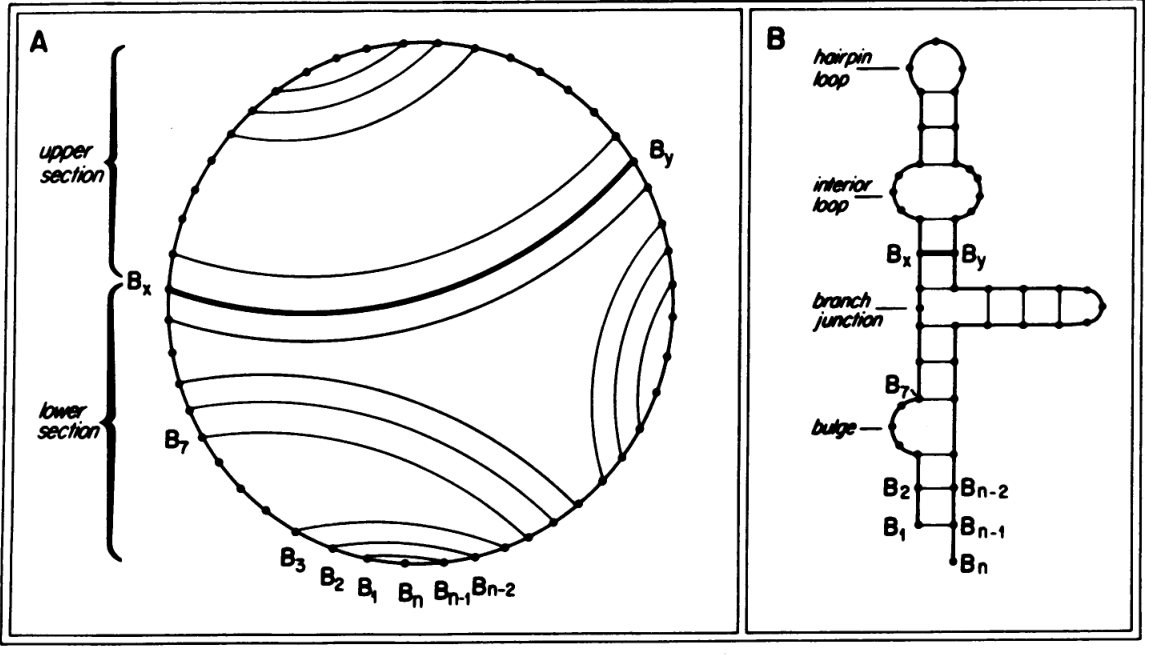
\includegraphics{nuss_rna}}
\end{center}
\caption{RNA secondary structure as described in the Nussinov algorithm.
Taken from the original publication \cite{nussinov1980fast}.}
\label{nuss_rna}
\end{figure}



Because of its dynamic programming
nature, this algorithm performs recursive decompositions of the RNA and builds
larger structures out of repeated substructures. A natural representation of this is
depicted in Figure \ref{nuss_rna}. Part A of Figure \ref{nuss_rna} shows bonds as arcs across a circular
graph. In it, we see the nested nature of the structures being explored by the
Nussinov algorithm. Part B shows how these structures translate to actual RNAs,
and how these appear in vivo. It also introduces the standard decompositions
of secondary structures, namely the hairpin loop, the interior loop, and the branch
junction or multi loop. Unlabelled in the diagram are stems; these are stacked
base pairings, for example $B1$, $Bn - 1$ and $B2$, $Bn - 2$.


\begin{equation} \label{eq:nuss_eq}
	M(i, j) = \max \left\lbrace A, B, C, D \right\rbrace 
\end{equation}
\[
A = M(i, j-1)
\]
\[
B = M(i+1, j)
\]
\[
C = M(i+1, j-1) + W(i, j)
\]
\[
D = \max \left\lbrace M(i, k) + M(k+1, j) \right\rbrace \: when \: i < k < j
\]



In the recurrence relation show in Equation \ref{eq:nuss_eq} the first two cases ($A$ and $B$) find the score associated with not allowing $i$ and $j$ to bond. The case $C$ conversely determines the score given that $i$ and $j$ are bonded. The final case $D$ computes the score associated with a bifurcation. A bifurcation here means decomposition of the RNA into two separate structures between. This recurrence relation implies a $O(N^3)$
worst case time complexity and a $O(N^2)$ space complexity, as an $O(N^2)$ state space (all combinations of $i$ and $j$) is explored
with a linear time recurrence relation. In the original algorithm a constant $p = 3$ was introduced that indicated the minimum size of a hair-pin loop as real RNAs typically do not have hair-pin loops of fewer bases. The recurrence relation presented here has also been modified for the sake of clarity (cases $A$ and $B$ can be merged into case $D$) but the logic of the algorithm is equivalent.


This algorithm can also be extended to accommodate a more advanced energy
model. Instead of weighting each bond equally they can be weighted
according to the proportion they are expected to contribute to the molecule’s
stability \cite{nussinov1980fast}. When considering the value of a bond, it might be given greater
weight if it adds to the formation of a stem (a stabilizing structure), or
given lower weight if it forms an internal loop or bulge as these generally
destabilize RNA molecules \cite{nussinov1980fast}. Unfortunately it is hard to find good values for
such weights, and determining which substructure a bond contributes to requires
backtracking in the modified algorithm presented by Nussinov \& Jacobson.

The reader should note that the Nussinov algorithm is old technology and is no longer used for the prediction of RNA secondary structures. I have presented it in detail here because it forms the basis for the most widely used algorithm today, which is shall thence discuss since it in turn is the basis for my own algorithms.


Soon after the work of Nussinov \& Jacobson, Zuker \& Stiegler \cite{zuker1981optimal}
described an altered version of the same algorithm which, instead of maximising
base pairs, minimized the free energy of the secondary structure. This was done
by introducing a number of thermodynamic rules for canonical structures like
hairpin loops, internal bulges, multiloops, unbonded base pairs, and stacked base
pairs. The algorithm is similar to the Nussinov algorithm
but adds another mutually recursive dynamic programming recurrence to inject
a complex and relatively comprehensive energy system. The original energy system used is borrowed from the work of Studnicka et al. \cite{studnicka1978computer} who presented a
complex algorithm which predicted similar RNA secondary structures, albeit with
much worse asymptotic and implementation complexities. 


\begin{figure}
\begin{center}
\scalebox{0.3}{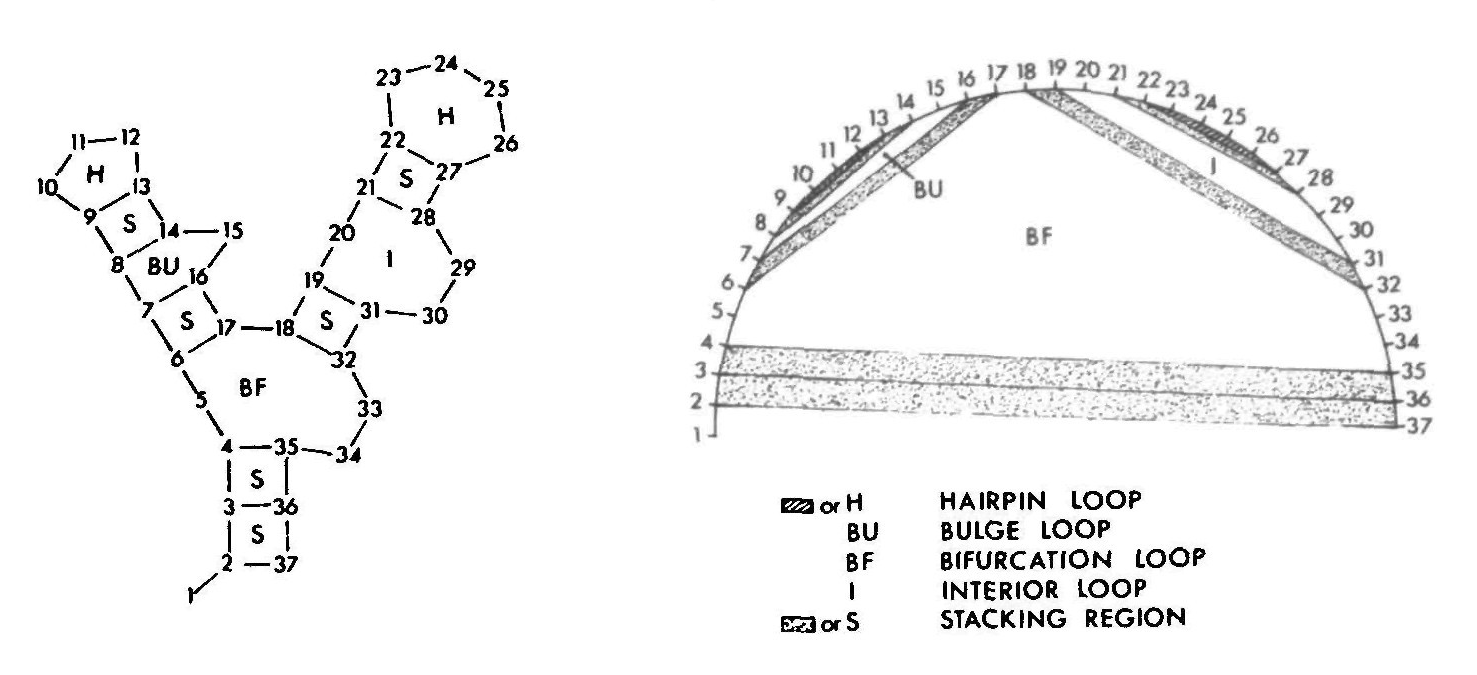
\includegraphics{figure4}}
\end{center}
\caption{Diagram of faces used in the Zuker algorithm. Taken from original
publication \cite{zuker1981optimal}.}
\label{zuk_struct}
\end{figure}

First I shall introduce some useful terminology which should clarify aspects of Zuker \& Stiegler’s
algorithm. The bases of an RNA molecule can be thought of as vertices in a
graph. Edges between such vertices can be represented as chords on a semicircular diagram (Figures \ref{nuss_rna} and \ref{zuk_struct}), such chords are not allowed to touch. A chord
is admissible if the bonds connected by it are chemically valid bonds, and an
admissible structure is a structure whose graph contains only admissible bonds.
Thence one can define a face of such a graph as any planar region bounded on all
sides; these faces represent the basic substructures of an RNA molecule \cite{zuker1981optimal}. The
folding algorithm of Zuker \& Stiegler considers such faces as the basic contributing factor to a molecule’s stability, unlike the algorithm of Nussinov \& Jacobson
which considers only individual bonds.


Let $E(F)$ represent the energy of a face $F$; impossible structures are given
an energy value of infinity, for example hairpin loops with less than three bases in the
intervening loop region. In addition let $V(i, j)$ be defined as the minimum free
energy of all structures in which bases $i$ and $j$ are bonded, and let $W(i, j)$ represent
the minimum free energy of all structures contained within bases $i$ and $j$ inclusive.
Note that for $W(i, j)$ there may or may not be a bond between bases $i$ and $j$. Also
if $i$ and $j$ cannot bond then $V(i, j) = \infty $. Finally note that $FH(i, j)$ represents a
hairpin loop structure from $i$ to $j$, and that $FL(i, j, i' , j' )$ is defined as the region
bounded by the bonds $i, j$ and $i', j'$. Examples of these decompositions are shown
diagrammatically in the right half of Figure \ref{zuk_struct}. The labelled regions show faces
in a semicircular graph representing a strand of RNA. In the accompanying left
half of the figure, the same RNA structure is shown as it would appear in a real
RNA rather than in a purely diagrammatic depiction.

\begin{equation} \label{eq:zuk_v1_eq}
V(i, j) = \min \left\lbrace E1, E2, E3 \right\rbrace
\end{equation}
$$E1 = E(FH(i, j))$$
$$E2 = \min \left\lbrace E(FL(i, j, i', j')) + V (i', j') \right\rbrace \: where \: i < i' < j' < j$$
$$E3 = \min \left\lbrace W (i + 1, i') + W (i' + 1, j − 1) \right\rbrace \: where \: i + 1 < i' < j - 2$$


As shown by the definition provided in Equation \ref{eq:zuk_v1_eq}, $V (i, j)$ is computed by minimizing
three cases. The first case considers the bond between $i$ and $j$ closing off a hairpin
loop (H in Figure \ref{zuk_struct}). The second accounts for cases in which $i$ and $j$ are bonded. This can result in a bulge (BU in Figure \ref{zuk_struct}), internal loop (I in Figure \ref{zuk_struct}), or the continuation of a stacking region (S in Figure \ref{zuk_struct}) between the
interior bond $i',j'$. The third and final case considers bifurcations
(BF in Figure \ref{zuk_struct})

\begin{equation} \label{eq:zuk_v1_eq2}
W (i, j) = \min \left\lbrace W(i + 1, j), W(i, j − 1), V(i, j), E4 \right\rbrace
\end{equation}
$$
E4 = \min \left\lbrace W (i, i') + W (i' + 1, j) \right\rbrace \: where \: i < i' < j - 1
$$

In Equation \ref{eq:zuk_v1_eq2} we show the recurrence for $W(i, j)$ as described by Zuker \& Stiegler.
Again there are three cases. The first two cases $W (i + 1, j)$ and $W(i, j − 1)$
should be thought of as a single case which consider situations in which there
is no bond between $i$ and $j$. This is similar to cases $A$ and $B$ from the Nussinov algorithm (Equation \ref{eq:nuss_eq}). The final case considers taking the bond from
$i$ to $j$. This final case allows for bifurcations in which two bonding pairs split
the structure into two sections. The final minimum free energy of the best structure is defined by $W(1, n)$, where $n$ is the length of the RNA molecule. It should
be noted that the free energy for small molecules (fewer than 6 nucleotides in length) can easily be
precomputed, and forms the base case of the given recurrence relations. Because of
its efficiency ($O(N^3)$ time and $O(N^2)$ space), robustness, and extensibility, this method,
even today, is still the most popular technique available. The most widely used packages for RNA secondary structure prediction are all implementations of the Zuker algorithm \cite{reuter2010rnastructure, lorenz2011viennarna}.


The Zuker algorithm suffers a major shortcoming, however. Because all bonding regions are assumed to be nested, it
cannot handle the case of `pseudoknots'. Pseudoknots are structures in which a bonding pair may have its first
base inside another bonding pair, and the other base outside said bonding pair.
In short, it is not properly nested. 

These structures are not common,
but have been experimentally verified in numerous RNAs \cite{taufer2009pseudobase}. In addition to this,
these kinds of structures also appear to perform useful biological functions. For
example, pseudoknots have been shown to allow frame shifting during translation
of proteins \cite{namy2006mechanical}. In layman’s terms, pseudoknots can change the way RNA is read
when being translated into protein. Such frame shifting is used extensively by
viruses, particularly HIV \cite{namy2006mechanical}. Unfortunately, the problem of finding optimal
structures with pseudoknots has been shown to be NP-Complete \cite{lyngso2000rna}.



\subsection{Pseudoknots}
In my investigation I did not consider the prediction of pseudoknotted RNA as they are uncommon. However I deem it important to understand how such structures could be integrated into the algorithms presented in this paper. As such, I have included a brisk overview of current pseudoknot prediction techniques.

Despite the problem being NP-Complete, in 1999 Rivas \& Eddy [20] introduced an ingenious dynamic
programming algorithm based on a new thermodynamic model encompassing pseudoknots. Their algorithm could predict a large set of pseudoknot classes using
O(N 6 ) time and O(N 4 ) memory. They generalised the Zuker method by us-
ing a gap matrix to represent regions being considered for bonding, rather than
the single continuous region used in the Zuker method. Because of its heavy
space and time requirements, this algorithm is used only sparingly in practice;
as such, other thermodynamic based methods for pseudoknot prediction have
been formulated based on similar principals. Deogun et al. [5] described an algo-
rithm which could handle a restricted class of pseudoknots (only those containing
non-recursive pseudoknots) in O(N 4 ) time and using O(N 3 ) space. Shortly after which Reeder \& Giegerich [19] presented an algorithm which could predict
only simple recursive pseudoknots which met their `canonization' criteria. While
seemingly restrictive, this did, in fact, predict a large array of pseudoknots accurately. 

In recent years, parallel algorithms have become more important for
achieving large speed-ups. In keeping with this, Guillaume \& Lavenier [22] implemented Zuker’s algorithm on the Graphics Processing Unit (GPU), yielding
a 17 fold speed-up despite the complex memory access pattern of the algorithm.
Thus far none of the pseudoknot capable algorithms have been implemented to
run on GPUs.


1.2.3 Accuracy
It is important to test and compare the accuracy of various prediction methods.
As such, well established nomenclature and techniques have been developed over
the history of RNA structure prediction. These methods are simple but effec-
tive. Usually accuracy is determined by comparing predicted structures to known
structures. True Positives (T P ) is defined as the number of base pairs which ap-
pear in both the predicted structure and the actual structure. False Positives
(F P ) is the number of base pairs in the predicted structure but not in the true
structure \cite{lorenz2011viennarna}. Similarly, False Negatives (F N ) is defined as the number of base
pairings in the reference structure but not present in the predicted structure \cite{lorenz2011viennarna}.
Using these terms one can defined sensitivity as the True Positive Rate (T P R),
or in other words the fraction of correctly predicted pairs [31].
TP
(1.1)
TP + FN
Precision, also known as Positive Predictive Value (P P V ), can also be calculated
using these values.
TPR =
PPV =
TP
TP + FP
(1.2)
RNAfold is one of the leading RNA folding algorithms, and is made available
as part of the Vienna RNA package \cite{lorenz2011viennarna}. At its heart it is an implementation
of the original dynamic programming algorithm first discovered by Zuker, albeit
with a more refined energy model. It is an extremely efficient implementation of
this algorithm, and is also one of the most accurate in terms of sensitivity and
PPV as compared to other implementations of the same algorithm \cite{lorenz2011viennarna}. When
Reeder \& Giegerich [19] first described their algorithm (implemented in the pack-
age pknotsRG) for pseudoknot prediction they compared it to RNAfold, and the
algorithm of Rivas \& Eddy [20] (implemented in the same package and hereafter
referred to as pknotsRE). Their algorithm generally had higher sensitivity than
9
both other methods, but it is worth noting that pknotsRE was extremely close,
despite being based on an outdated energy model. This is possibly explained by
the fact that it is a more general and thus a more powerful algorithm. RNAfold
lagged behind both in sensitivity, but executed orders of magnitude faster. In-
deed, it has been shown to have excellent accuracy for smaller RNAs containing
no pseudoknots while also exhibiting unrivalled computation speed \cite{lorenz2011viennarna}.


1.3 Alternative Techniques
1.3.1 Context Free Grammars
RNA sequences and their secondary structures can be represented as context free
grammars. Various production rules output different internal structures (such as
hairpin loops, or internal bulges), with the terminals producing the bases A, U, G,
and C. This is a fundamentally different approach to those discussed previously,
however it can, in fact, use the same thermodynamic energy model. Stochas-
tic Context Free Grammars (SCFGs) can be used to encode the plausibility of
structures, and thus find the most plausible looking structure using a thermo-
dynamic model [21]. In addition, these kinds of algorithms can be trained to
incorporate statistical information such as phylogenetic similarity, or machine
learned parameters [21]. These kinds of methods have trouble with pseudoknots,
as non-nested structures are not compatible with typical context free grammars.
One notable workaround was applied by Kato, Seki, and Kasami [10], who used
multiple context free grammars to model pseudoknots. This approach, however,
increases the time and space requirements of the typical algorithm.
The greatest strength of context free grammar based approaches is that they
can diverge from the use of free energy entirely. This is advantageous as using
a physics based model–such as free energy minimization–requires a large volume
of experimentally verified parameters. For this reason, many parameters are of-
ten not included in such models because they cannot be quantified empirically.
The energy value of multibranch loops, for example, is not known and is usually
guessed at in modern RNA prediction algorithms. Likewise, the inter-structural
interactions of hairpin loops, bulges, multibranch loops, and internal loops has
not been quantified experimentally and is thus not used as a free energy param-
eter. CONTRAfold [6] was one of the first SCFG based algorithms to achieve
comparable performance to Zuker-like free energy minimization methods. It does
away with the notion of free energy minimization altogether and instead uses a
set of trained parameters based on conditional log-linear models. CONTRAfold
achieved an average prediction sensitivity higher than RNAfold, and also higher
10
than that of Mfold [32] (an RNA prediction package similar to RNAfold). It
is important, however, to remember that none of these approaches are able to
model pseudoknots.

1.3.2 Soft Computing
The use of soft computing techniques has also yielded some success in the predic-
tion of RNA secondary structure. Koessler et al. [11] modeled RNA structures
as a tree of internal structures, then used artificial neural networks to recognize
which of these trees appeared most RNA like. The trees were generated by con-
structing basic secondary structures and combinatorially merging them together
to form many trees, each of which was represented as a vector of simpler trees.
This vector was used as the input to the neural network. This kind of combina-
torial blending of RNA stems is also common to genetic algorithms. Indeed, this
is precisely the starting point of Van Batenburg, Gultyaev, and Pleij [28], who
used a simple genetic algorithm to predict secondary structure. Their algorithm
starts by computing an array of all possible stems; each genome is represented
as a binary string where 1 indicates a stem is in the candidate structure, and 0
indicates that it is not. Their genetic algorithm proceeds by seeding the genomes
with random bits, then, in a series of generation steps, performs typical binary
mutation, crossover and breeding, conserving and selectively breeding the fittest
solutions. Fitness was defined in their algorithm as the summed total length
(number of bases) of all stems, and in an improved version, the summed stacking
free energy reduction of all stems.

Unfortunately they discovered a problem with this approach: the population
contained a relatively large portion of zero fitness individuals. This was because
many combinations of stems are incompatible with each other, yielding impossible
structures. Instead of giving these structures zero fitness, they altered their algo-
rithm slightly to disallow merging for any stems that created an invalid structure.
In addition to this, they also explored an important advantage of genetic algo-
rithms for RNA secondary structure prediction: that of kinetic folding. Kinetic
folding is the hypothesis that some RNAs, particularly large ones, have a rugged
energy landscape and, because of the incremental process of transcription and
folding (which happen simultaneously), become stuck in suboptimal areas during
folding [28, 27]. The algorithm of Van Batenburg, Gultyaev, and Pleij simulated
this process by limiting the size of stems that could contribute to a genome, and
increasing this size over time until the length of the RNA was reached. This
single modification to their algorithm yielded the greatest improvement in pre-
dictive power. It should also be noted that it could also predict pseudoknots, as
the algorithm did not force stems to be nested. Despite this, their approach was
still less accurate than the dynamic programming approaches they compared it
to. This was most likely because their energy model was puerile in comparison,
rather than because the algorithm was flawed.


Indeed, Wiese, Deschenes, and Hendriks [30] recently introduced an improved
genetic algorithm based on the same principles as that of Van Batenburg, Gultyaev,
and Pleij, which instead used an advanced energy model for fitness. They then
demonstrated that it outperformed the popular dynamic programming algorithm
Mfold [32], which uses a similarly complex model. Genetic algorithms for RNA
secondary structure prediction have also been implemented on massively parallel
architectures. Shapiro et al. [23] reported on implementations for both Single
Instruction, Multiple Data (SIMD) architectures, and Multiple Instruction, Mul-
tiple Data MIMD architectures. These algorithms used several populations, and
treated each population as an island which evolved separately and therefore con-
currently. These islands would occasionally share their fittest solutions, which
allowed the algorithm to converge on a globally optimal solution. An interesting
observation is that, in recent years, many consumer computers have powerful
SIMD architectures in the form of their GPUs. While this avenue has already
been explored for Zuker’s algorithm [22], there is, as yet, no GPU implementation
of a genetic algorithm for RNA folding.

1.4 Locally Optimal Structure Prediction
DNA sequences, unlike typical RNA molecules, are very large indeed. Usually
on the order of hundreds of megabytes of data. Such sequences contain DNA
subsequences that code for RNAs. Functionally important RNAs typically have
a recognizable secondary structure. When searching a large genome for func-
tional RNAs, one could use a sliding window of fixed size to find locally optimal
structures. This might be done by running a typical cubic time algorithm like
RNAfold or Mfold at every window location. Let L be defined as the chosen
window size, and N represent the length of the RNA. This leads to a total com-
plexity of O(N L3 ). While not prohibitive, this becomes intractable for many
genomes, which are typically extremely large–millions or billions of bases. In
2004, Hofacker, Priwitzer, and Stadler [8] provided an excellent insight and were
able to lower this bound to O(N L2 ), making it possible to scan large genomes
for interesting RNA secondary structure motifs. This was achieved by using the
dynamic programming table from the previous step to quickly fill the table for
the next window in quadratic time; because consecutive windows overlap, pre-
ceding information can be meaningfully used in each forward computational step.
As a result it requires only a single table of size O(L2 ), and as such its mem-
12
ory complexity is only O(N + L2 ). Later, in 2009, Horesh et al. [9] managed
to lower the expected time bound to O(N L) under the assumption that one is
folding RNAs that are typical of naturally occurring sequences. This complex-
ity bound was experimentally verified, and their algorithm was shown to clearly
outperform that of Hofacker, Priwitzer, and Stadler. Clearly good algorithms are
available for the folding of consecutive RNA windows. For even a modest size
RNA, such algorithms perform orders of magnitude faster than holistic secondary
structure prediction algorithms, with the major caveat of not actually predicting
a complete secondary structure, but only a set of locally optimal structures.





The {\tt cshonours} files are located in:
\begin{verbatim}
/cslinux/cstex/local
\end{verbatim}

In order to use the {\tt cshonours} class you need to tell \TeX\ how
to find it. To do this simply add the following to your shell resource
file (ie.\ {\tt .zshrc}, {\tt .bashrc}, etc):
\begin{verbatim}
export TEXINPUTS=$TEXINPUTS:.:/cslinux/cstex//
\end{verbatim}
(The double-slash \verb!//! tells \TeX\ to search the tree from this
point.) Then open a new shell window to run \LaTeX\ in.

If you are using a machine that doesn't mount {\tt cslinux} or a
stand-alone system such as a home machine, you can take a copy of the
{\tt cshonours.cls} file and put it on your own machine. Please copy
the class file directly from the original in the above directory to
make sure you have an unadulterated copy.

Once you have told \TeX\ how to find the class file, the easiest way
to get started is to copy this example file, {\tt cshonours.tex}, and
the accompanying example bibliography file, {\tt cshonours.bib}, from
the above directory, give them a new name, and start modifying the text.

\section{What does it all mean?}
\label{code}

The example file is pretty self explanatory, but here's a little
elucidation for those who are interested.

\begin{verbatim}
\documentclass{cshonours}
\end{verbatim}
\ldots tells \LaTeX\ to use the {\tt cshonours} class. The commands
between here and the \verb!\begin{document}! command are known as the
{\em preamble\/} of the latex document. Font size is automatically set
to 12pt in this class.

\begin{verbatim}
\bibliographystyle{acm}
\end{verbatim}
\ldots sets the bibliography style. Default is the style used in
Transactions of the ACM.

\begin{verbatim}
\usepackage{graphics}  %optional
\end{verbatim}
\ldots this is only needed if you want to include postscript images.

\begin{verbatim}
\title{The Honours Dissertation Class for \LaTeX2e}
\author{Cara MacNish}
\end{verbatim}
\ldots same as usual.

\begin{verbatim}
\keywords{Honours, report preparation, \LaTeX}
\categories{A.2, I.7.2}
\end{verbatim}
\ldots keywords and Computing Reviews classification numbers. These
will be put at the bottom of the abstract page.

\begin{verbatim}
\begin{document}
\end{verbatim}
\ldots so much for the preamble, now we start the document proper.

\begin{verbatim}
\maketitle
\end{verbatim}
\ldots produces the title page using the title and author stored
earlier. Unlike the standard {\tt report} class it also starts roman
page numbering.

\begin{verbatim}
\begin{abstract}
This is a short report...
\end{abstract}
\end{verbatim}
\ldots produces the abstract page, including the keywords and
categories stored earlier.

\begin{verbatim}
\begin{acknowledgements}
This style is designed...
\end{acknowledgements}
\end{verbatim}
\ldots produces the acknowledgements page.

\begin{verbatim}
\tableofcontents
\listoftables  %optional
\listoffigures  %optional
\end{verbatim}
\ldots you guessed it! \verb!\listoftables! and \verb!listoffigures!
can be omitted if you have no tables or figures respectively.

\begin{verbatim}
\chapter{The Honours Dissertation Style Guide}
\end{verbatim}

\ldots and so the first chapter begins. Unlike the standard {\tt
report} class the first \verb!\chapter! command also switches
pagenumbering to arabic.

The main body is created using the usual \LaTeX\ commands. At the end
we come to:

\begin{verbatim}
\appendix
\end{verbatim}
\ldots starts off the appendices.

\begin{verbatim}
\bibliography{cshonours}
\end{verbatim}
\ldots puts in the bibliography, generated in this case from the
file {\tt cshonours.bib}.


\section{Carrying on\ldots}

The rest of the document proceeds in the usual way, with all standard
\LaTeX\ commands available. These are described in~\cite{bible}, which
is written by the author of \LaTeX, Leslie Lamport, and commonly known
as the \LaTeX\ ``Bible''.

For those who are feeling ambitious, a wealth of contributed
packages, some of which are included in our distribution, and some of
which you would need to download yourself, are described
in~\cite{doggie}, commonly known as the ``Doggie Book''.


\section{Including Postscript Files}

Most drawing packages (such as {\tt xfig} and {\tt xpaint}) and image
manipulation packages (such as {\tt xv} and {\tt gimp}) allow you to
save your work as (encapsulated) postscript, which can be easily
included in your \LaTeX\ document. The recommended (and simplest!) way
of doing this is by including the command \verb!\usepackage{graphics}!
in the preamble (see Section~\ref{code}) and then include the
postscript file using the \verb!\includegraphics! command.

\begin{figure}
\begin{center}

\includegraphics{gnu}
\end{center}
\caption{This is a Gnu.}
\label{gnu}
\end{figure}

For example, Figure~\ref{gnu} shows a Gnu, produced by the following code:
\begin{verbatim}
\begin{figure}
\begin{center}

\includegraphics{gnu}
\end{center}
\caption{This is a Gnu.}
\label{gnu}
\end{figure}
\end{verbatim}

\begin{figure}
\begin{center}
\scalebox{0.6}{
\includegraphics{gnu}}
\end{center}
\caption{This is a smaller Gnu.}
\label{smallergnu}
\end{figure}

You can scale graphics using the \verb!\scalebox! command. For
example, Figure~\ref{smallergnu} shows a smaller Gnu, produced as follows:
\begin{verbatim}
\begin{figure}
\begin{center}
\scalebox{0.6}{
\includegraphics{gnu}}
\end{center}
\caption{This is a smaller Gnu.}
\label{smallergnu}
\end{figure}
\end{verbatim}


\section{Producing Postscript Output}

\LaTeX\ produces a {\tt .dvi} file which you can convert to postscript
using {\tt dvips}. If you have included encapsulated postscript figures the
bounding boxes of those figures sometime confuse the printing
routines. To overcome this it is recommended you use the {\tt -K}
option to strip bounding box comments out. The full recommended format
is:

\begin{verbatim}
dvips -K -f myfile.dvi > myfile.ps
\end{verbatim}

To save typing I just use a simple script for
all my {\LaTeX}ing. Just create a file, called say {\tt laps}, containing something like:
\begin{verbatim}
latex $1
dvips -K -o $1.ps $1.dvi
\end{verbatim}
Then make it executable, run \LaTeX\ with the command
\begin{verbatim}
laps myfile
\end{verbatim}
and view with ghostview (with ``State'' set to ``Watch file'').

\section{Producing PDF}

If you prefer PDF output you can produce this using {\tt
pdfelatex}. This does not use {\tt dvi} as an intermediary so you just
say:
\begin{verbatim}
pdfelatex myfile
\end{verbatim}

Note that any graphics you include must also be in
suitable PDF. There are conversion programs, such as {\tt ps2pdf}, but
I've found they often don't work well. It is better to produce the
graphics directly in {\tt pdf}.

I've also found that {\tt pdf} viewers don't tend to refresh well, so
that you need to keep opening the file. As a result I tend to
postscript where possible.


\section{Emacs and \LaTeX}

Gnu Emacs and Xemacs recognise both {\tt .tex} and {\tt .bib} files,
and provide a number of tools for preparing them. For example you can
select {\tt .bib} entry templates from a drop-down menu. Simple
commands like \verb!C-c C-e! (puts in the \verb!\end! command to
finish an environment) save lots of typing.


\section{Appendices}

After the main body comes the appendices. See Appendix~\ref{appa} and
Appendix~\ref{appb}.

\section{Bibliography}

Finally, the bibliography can be produced automatically from a {\tt .bib} file
using {\tt bibtex} in the usual way. This is described
in~\cite{bible}. 

The bibliography is the only change from the \LaTeX 2.09 {\tt
cshonours} style file. The bibliography now comes after the
appendices, in line with printed books, and uses alphanumeric citation
tags to make reading (and marking) easier.


\appendix

\chapter{Original Honours Proposal}
\label{appa}

You must include as your first appendix an exact copy (in wording) of
your original project proposal. This aids other readers to establish
what was the initial focus of the project.

\chapter{Another Appendix}
\label{appb}

Other appendices might include pseudocode 
for your implementation, a Users Manual, an important data file, etc. 

\bibliography{cshonours}

\end{document}


